\documentclass{article}

\usepackage{fancyhdr}
\usepackage{extramarks}
\usepackage{amsmath}
\usepackage{amsthm}
\usepackage{amssymb}
\usepackage{amsfonts}
\usepackage{tikz}
\usepackage[plain]{algorithm}
\usepackage{algpseudocode}
\usepackage{float} 

\usetikzlibrary{automata,positioning}

%
% Basic Document Settings
%

\topmargin=-0.45in
\evensidemargin=0in
\oddsidemargin=0in
\textwidth=6.5in
\textheight=9.0in
\headsep=0.25in

\linespread{1.1}

\pagestyle{fancy}
\lhead{\hmwkAuthorName}
\chead{\hmwkClass\ \hmwkTitle}
%\chead{\hmwkClass\ (\hmwkClassInstructor\ \hmwkClassTime): \hmwkTitle}
\rhead{\firstxmark}
\lfoot{\lastxmark}
\cfoot{\thepage}

\renewcommand\headrulewidth{0.4pt}
\renewcommand\footrulewidth{0.4pt}

\setlength\parindent{0pt}

%
% Create Problem Sections
%

\newcommand{\enterProblemHeader}[1]{
    \nobreak\extramarks{}{Problem \arabic{#1} continued on next page\ldots}\nobreak{}
    \nobreak\extramarks{Problem \arabic{#1} (continued)}{Problem \arabic{#1} continued on next page\ldots}\nobreak{}
}

\newcommand{\exitProblemHeader}[1]{
    \nobreak\extramarks{Problem \arabic{#1} (continued)}{Problem \arabic{#1} continued on next page\ldots}\nobreak{}
    \stepcounter{#1}
    \nobreak\extramarks{Problem \arabic{#1}}{}\nobreak{}
}

\setcounter{secnumdepth}{0}
\newcounter{partCounter}
\newcounter{homeworkProblemCounter}
\setcounter{homeworkProblemCounter}{1}
\nobreak\extramarks{Problem \arabic{homeworkProblemCounter}}{}\nobreak{}

%
% Homework Problem Environment
%
% This environment takes an optional argument. When given, it will adjust the
% problem counter. This is useful for when the problems given for your
% assignment aren't sequential. See the last 3 problems of this template for an
% example.
%
\newenvironment{homeworkProblem}[1][-1]{
    \ifnum#1>0
        \setcounter{homeworkProblemCounter}{#1}
    \fi
    \section{Problem \arabic{homeworkProblemCounter}}
    \setcounter{partCounter}{1}
    \enterProblemHeader{homeworkProblemCounter}
}{
    \exitProblemHeader{homeworkProblemCounter}
}

%
% Homework Details
%   - Title
%   - Due date
%   - Class
%   - Section/Time
%   - Instructor
%   - Author
%

\newcommand{\hmwkTitle}{Homework\ \#2}
\newcommand{\hmwkDueDate}{February 8, 2022}
\newcommand{\hmwkClass}{EECS 545 Machine Learning}
\newcommand{\hmwkClassTime}{Section A}
\newcommand{\hmwkClassInstructor}{Professor Honglak Lee}
\newcommand{\hmwkAuthorName}{\textbf{Yuang Huang}}
\newcommand{\hmwkUninameName}{\textbf{yahuang@umich.edu}}

%
% Title Page
%

\title{
    \vspace{2in}
    \textmd{\textbf{\hmwkClass:\ \hmwkTitle}}\\
    \normalsize\vspace{0.1in}\small{Due\ on\ \hmwkDueDate\ at 12pm}\\
    \vspace{0.1in}\large{\textit{\hmwkClassInstructor\ \hmwkClassTime}}
    \vspace{3in}
}

\author{\hmwkAuthorName\\
\hmwkUninameName}
\date{}

\renewcommand{\part}[1]{\textbf{\large Part \Alph{partCounter}}\stepcounter{partCounter}\\}

%
% Various Helper Commands
%

% Useful for algorithms
\newcommand{\alg}[1]{\textsc{\bfseries \footnotesize #1}}

% For derivatives
\newcommand{\deriv}[1]{\frac{\mathrm{d}}{\mathrm{d}x} (#1)}

% For partial derivatives
\newcommand{\pderiv}[2]{\frac{\partial}{\partial #1} (#2)}

% Integral dx
\newcommand{\dx}{\mathrm{d}x}

% Alias for the Solution section header
\newcommand{\solution}{\textbf{\large Solution}}

% Probability commands: Expectation, Variance, Covariance, Bias
\newcommand{\E}{\mathrm{E}}
\newcommand{\Var}{\mathrm{Var}}
\newcommand{\Cov}{\mathrm{Cov}}
\newcommand{\Bias}{\mathrm{Bias}}

\begin{document}

\maketitle

\pagebreak

\begin{homeworkProblem}
    \large {Logistic regression}
    \\
    \textbf{Solution}

    \textbf{Part a:} Hessian $H$ 

    \begin{equation}
    l(\mathbf{w}) = \sum_{i=1}^{N}y^{(i)}\log h(\mathbf{x}^{(i)}) + (1 - y^{(i)})\log (1 - h(\mathbf{x^{(i)}})),
    \label{eq1}
    \end{equation}
    where $h(\mathbf{x}) = \sigma(\mathbf{w^Tx}) = \frac{1}{1+\exp(-\mathbf{w^Tx})}$ and we denote that $pred = \mathbf{w^Tx}$.

    Then we assume that: 
    \begin{equation}
    l_i(\mathbf{w}) = y^{(i)}\log \sigma(pred^{(i)}) + (1 - y^{(i)})\log (1 - \sigma(pred^{(i)})),
    \label{eq2}
    \end{equation}
    where we know that $\frac{\partial pred}{\partial \mathbf{w}} = \mathbf{x^T}$ and $\frac{\partial pred}{\partial \mathbf{w^T}} = \mathbf{x}$.\\
    It can be shown that:
    \begin{equation}
    \begin{aligned}
    \nabla l_i(\mathbf{w})&= \frac{y^{(i)}x^{(i)}}{\sigma({pred^{(i)}})} - \frac{(1 - y^{(i)})x^{(i)}}{(1 - \sigma(pred^{(i)}))}\\
    &= y^{(i)}x^{(i)}(1 - \sigma({pred^{(i)}})) - (1 - y^{(i)})x^{(i)}\sigma(pred^{(i)})\\
    &= x^{(i)}y^{(i)} -x^{(i)}\sigma{(pred^{(i)})}
    \label{eq3}
    \end{aligned}
    \end{equation}
    Then we can be write:
    \begin{equation}
    \begin{aligned}
    H^{(i)} = \nabla^2 l_i(\mathbf{w})&= -x^{(i)}x^{(i)^T}\frac{1}{1 + \exp(pred^{(i)})}\frac{\exp(pred^{(i)})}{1 + \exp(pred^{(i)})}\\
    &= -x^{(i)}x^{(i)^T}\sigma(pred^{(i)})(1 - \sigma(pred^{(i)}))
    \label{eq4}
    \end{aligned}
    \end{equation}
    so the Hessian $H$ is written by:
    \begin{equation}
    \begin{aligned}
    H = -\mathbf{xRx^T}
    \label{eq5}
    \end{aligned}
    \end{equation}
    where $R$ is the diagnal matrix that the diagnal elements are $\sigma(pred^{(i)})(1 - \sigma(pred^{(i)}))$.
    Thus,
    \begin{equation}
    \begin{aligned}
    \mathbf{z^T}H\mathbf{z} &= -\mathbf{zxRx^Tz^T}\\
    &= -||\mathbf{z^TRX}||^2 \leq 0.
    \label{eq6}
    \end{aligned}
    \end{equation}
    So it is shown that Hessian $H$ is negative semi-definite 
    and thus $l$ is concave and has no local maxima other than the global one.
    \pagebreak

    \textbf {Part b:} 

    Since Hessian $H = -\mathbf{xRx^T}$, and $R$ depends on $w$ (and vice versa), we get iterative reweighted least squares (IRLS)
    \begin{equation}
    \begin{aligned}
        R_{ii} &= \sigma(pred^{(i)})(1 - \sigma(pred^{(i)}))\\
        &= h^{(n)}(1 - h{(n)}),
    \end{aligned}
    \end{equation}
    where
    \begin{equation}
    \begin{aligned}
        \mathbf{w}^{(new)} &= \mathbf{(\Phi^TR\Phi)}^{-1}\mathbf{\Phi^TRz}\\
        \mathbf{z} &= \mathbf{\Phi w}^{(old)} - \mathbf{R^{-1}(h - y)}.
    \end{aligned}
    \end{equation}

    Initialize Newton's method with $\mathbf{w} = \mathbf{0}$, after iterations, $\mathbf{w}$ are shown as followed:

    $\bullet \quad w_0 = -1.84922892$

    $\bullet \quad w_1 = -0.62814188$

    $\bullet \quad w_2 = 0.85846843$

    So the slope term of the decision boundary is $- \frac{w_1}{w_2} = 0.73170061$ and the itercept term of the decision 
    boundary is $- \frac{w_0}{w_2} = 2.15410241$.\\

    \textbf{Part c:} 
    \begin{figure}[H]  
    \centering  
    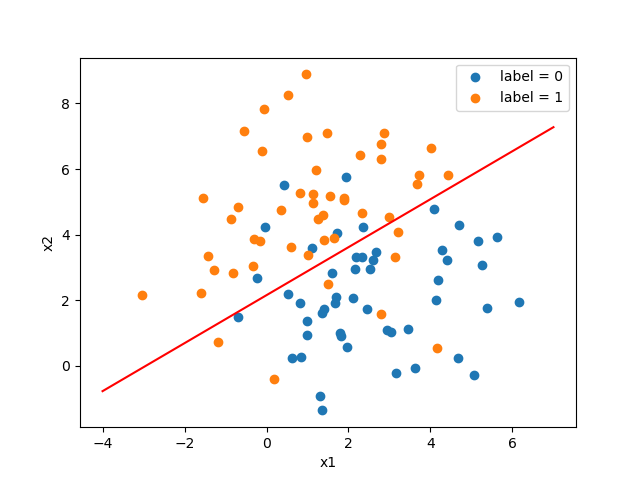
\includegraphics[width=4in,height=3.2in]{hw2_q1_c.png} 
    \caption{The training data and the decision boundary fit by logistic regression} 
    \label{Fig1}
    \end{figure}
    As shown in Fig. \ref{Fig1}, we can see the training data and the decision boundary fit by logistic regression.
    It obviously has a good classification effect.

\end{homeworkProblem}

\pagebreak

\begin{homeworkProblem}
    \large Softmax Regression via Gradient Ascent\\

    \textbf{Solution}

    \textbf{Part a:}\\
     \begin{equation}
     \begin{aligned}
    \nabla_{\mathbf{w_m}} l(\mathbf{w}) = \sum_{i=1}^{N}\phi (\mathbf{x}^{(i)}){\left [\mathbf{I}(y^{(i)} = m) - \frac{\exp(\mathbf{w}^{T}_{m}\phi(\mathbf{x}^{(i)}))}{1 + \sum_{j = 1}^{K -1} \exp(\mathbf{w}^T_{j}\phi(\mathbf{(x)}^{(i)}))}\right] },
    \label{eq8}
    \end{aligned}
    \end{equation}
    and we know :
    \begin{equation}
    \begin{aligned}
    p(y = k|\mathbf{x}, \mathbf{w}) &= \frac{\exp(\mathbf{w}^{T}_{m}\phi(\mathbf{x}^{(i)}))}{1 + \sum_{j = 1}^{K -1} \exp(\mathbf{w}^T_{j}\phi(\mathbf{(x)}^{(i)}))},\\
    l(\mathbf{w}) &= \sum_{i = 1}^{N}\sum_{k = 1}^{K}\log (\left [p(y^{(i)} = k|\mathbf{x}^{(i)}, \mathbf{w})\right]^{\mathbf{I}(y^{(i) = k})}).
    \label{eq9}
    \end{aligned}
    \end{equation}
    with (\ref{eq8}) and (\ref{eq9}), we can get:
    \begin{align}
    \notag
    \nabla_{\mathbf{w_m}} l(\mathbf{w}) &= \nabla_{\mathbf{w}} \sum_{i=1}^{N}\sum_{k=1}^{K}  \mathbf{I}(y^{(i)} = k){\left [ \mathbf{w}^{T}_{m}\phi(\mathbf{x}^{(i)})- \log (1 + \sum_{j = 1}^{K -1} \exp(\mathbf{w}^T_{j}\phi(\mathbf{(x)}^{(i)}))\right]) }\\ \notag
    &= \sum_{i=1}^{N} \nabla_{\mathbf{w}} \sum_{k=1}^{K}  \mathbf{I}(y^{(i)} = k){\left [ \mathbf{w}^{T}_{m}\phi(\mathbf{x}^{(i)})- \log (1 + \sum_{j = 1}^{K -1} \exp(\mathbf{w}^T_{j}\phi(\mathbf{(x)}^{(i)}))\right]) }\\ \notag
    &= \sum_{i=1}^{N} \Big(\nabla_{\mathbf{w}} \sum_{k\neq m}^{K}  \mathbf{I}(y^{(i)} = k){\left [ \mathbf{w}^{T}_{m}\phi(\mathbf{x}^{(i)})- \log (1 + \sum_{j = 1}^{K -1} \exp(\mathbf{w}^T_{j}\phi(\mathbf{(x)}^{(i)}))\right]) }\\ \notag
    &+\nabla_{\mathbf{w}} \mathbf{I}(y^{(i)} = m) {\left [ \mathbf{w}^{T}_{m}\phi(\mathbf{x}^{(i)})- \log (1 + \sum_{j = 1}^{K -1} \exp(\mathbf{w}^T_{j}\phi(\mathbf{(x)}^{(i)}))\right]) } \Big) \\
    &= \sum_{i=1}^{N} \Big(- \nabla_{\mathbf{w}} \sum_{k\neq m}^{K}  \mathbf{I}(y^{(i)} = k){\left [ \log (1 + \sum_{j = 1}^{K -1} \exp(\mathbf{w}^T_{j}\phi(\mathbf{(x)}^{(i)}))\right]) }\\ \notag
    &+ \mathbf{I}(y^{(i)} = m) {\left [ \phi(\mathbf{x}^{(i)})- \nabla_{\mathbf{w}} \log (1 + \sum_{j = 1}^{K -1} \exp(\mathbf{w}^T_{j}\phi(\mathbf{(x)}^{(i)}))\right]) } \Big)\\ \notag
    &= \sum_{i = 1}^{N} \Big( \mathbf{I}(y^{(i)} = m) \phi(\mathbf{x}^{(i)})- \nabla_{\mathbf{w}} \log (1 + \sum_{j = 1}^{K -1} \exp(\mathbf{w}^T_{j}\phi(\mathbf{(x)}^{(i)})))  \Big)\\ \notag
    &= \sum_{i = 1}^{N} \phi(\mathbf{x}^{(i)}) \Big( \mathbf{I}(y^{(i)} = m) - \nabla_{\mathbf{w}} \frac{\exp(\mathbf{w}^T_{j}\phi(\mathbf{(x)}^{(i)}))} {(1 + \sum_{j = 1}^{K -1} \exp(\mathbf{w}^T_{j}\phi(\mathbf{(x)}^{(i)})))}  \Big)\\ \notag
    & = \sum_{i = 1}^{N} \phi(\mathbf{x}^{(i)}) \Big(\mathbf{I}(y^{(i)} = m) - p(y^{(i)} = m|\mathbf{x}^{(i)}, \mathbf{w}) \Big)
    \label{eq10}
    \end{align}
    \textbf{Part b:}\\
    After 500 iterations, the accuracy of the predictions from my model is 0.98 and 
    the accuracy of the predictions from sklearn's LogisticRegression is 0.92.\\
    
    The predictions from sklearn's LogisticRegression:

    [2. 3. 1. 1. 1. 2. 2. 1. 1. 3. 2. 3. 1. 2. 3. 2. 1. 1. 2. 1. 3. 2. 3. 3.
    1. 3. 3. 3. 3. 3. 2. 3. 2. 1. 3. 2. 1. 2. 3. 1. 1. 1. 1. 2. 1. 2. 2. 2.
    3. 3.] \\

    The predictions from my model (500iter): 
    
    [2. 3. 1. 1. 1. 2. 3. 1. 1. 3. 2. 3. 1. 2. 3. 2. 1. 1. 2. 1. 3. 2. 3. 3.
    1. 3. 3. 3. 3. 3. 2. 3. 2. 1. 3. 2. 1. 2. 3. 1. 1. 1. 1. 2. 1. 2. 3. 3.
    3. 3.] \\

    The result of the predictions from sklearn's LogisticRegression: 
    
    [ True  True  True  True  True  True False  True  True  True  True  True
    True  True  True  True  True  True  True  True  True  True  True  True
    True  True  True False  True  True  True  True  True  True  True  True
    True  True  True  True  True  True  True  True  True  True False False
    True  True] \\
    
    The predictions from my model (500iter): 
    
    [ True  True  True  True  True  True  True  True  True  True  True  True
    True  True  True  True  True  True  True  True  True  True  True  True
    True  True  True False  True  True  True  True  True  True  True  True
    True  True  True  True  True  True  True  True  True  True  True  True
    True  True] \\
    
    \begin{figure}[H]  
        \centering  
        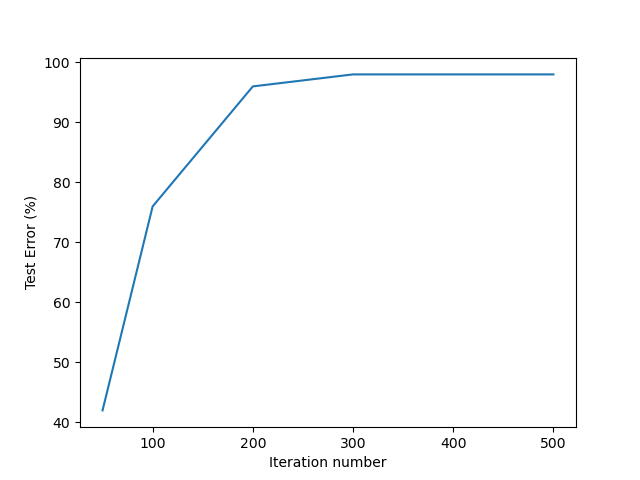
\includegraphics[width=4in,height=3.2in]{hw2_q2_c.png} 
        \caption{the test of error with respect to size of training sets} 
        \label{Fig3}
    \end{figure}
    As shown in Fig. \ref{Fig3}, we can see the the test of error with respect to iteration numbers.
    When the iteration number is 200, the performance is better than sklearn's LogisticRegression.


    


    

    
\end{homeworkProblem}

\pagebreak

\begin{homeworkProblem}
    \large Gaussian Discriminate Analysis\\

    \textbf{Solution}

    \textbf{Part a:}\\
    \begin{equation}
    \begin{aligned}
    &p(y = 1|\mathbf{x}^{(i)}) = \frac{p(\mathbf{x}^{(i)}|y = 1)p(y = 1)}{p(\mathbf{x}^{(i)})}\\
    &= \frac{p(\mathbf{x}^{(i)}|y = 1)p(y = 1)}{p(\mathbf{x}^{(i)}|y = 1)p(y = 1) + p(\mathbf{x}^{(i)}|y = 0)p(y = 0)}\\
    &= \frac{\frac{1}{(2\pi)^{\frac{M}{2}}|\Sigma|^{\frac{1}{2}}} \exp(-\frac{1}{2}(\mathbf{x}^{(i)} - \mu_1)^T\Sigma^{-1}(\mathbf{x}^{(i)} - \mu_1))\phi}{\frac{1}{(2\pi)^{\frac{M}{2}}|\Sigma|^{\frac{1}{2}}} \exp(-\frac{1}{2}(\mathbf{x}^{(i)} - \mu_1)^T\Sigma^{-1}(\mathbf{x}^{(i)} - \mu_1))\phi + \frac{1}{(2\pi)^{\frac{M}{2}}|\Sigma|^{\frac{1}{2}}} \exp(-\frac{1}{2}(\mathbf{x}^{(i)} - \mu_0)^T\Sigma^{-1}(\mathbf{x}^{(i)} - \mu_0))(1 - \phi)}\\
    & = \frac{\exp(-\frac{1}{2}(\mathbf{x}^{(i)} - \mu_1)^T\Sigma^{-1}(\mathbf{x}^{(i)} - \mu_1))\phi}{ \exp(-\frac{1}{2}(\mathbf{x}^{(i)} - \mu_1)^T\Sigma^{-1}(\mathbf{x}^{(i)} - \mu_1))\phi +  \exp(-\frac{1}{2}(\mathbf{x}^{(i)} - \mu_0)^T\Sigma^{-1}(\mathbf{x}^{(i)} - \mu_0))(1 - \phi)}\\
    & = \frac{1}{1 + \frac{\exp(-\frac{1}{2}(\mathbf{x}^{(i)} - \mu_1)^T\Sigma^{-1}(\mathbf{x}^{(i)} - \mu_1))\phi}{\exp(-\frac{1}{2}(\mathbf{x}^{(i)} - \mu_0)^T\Sigma^{-1}(\mathbf{x}^{(i)} - \mu_0))(1 - \phi)}}
    \label{eq11}
    \end{aligned}
    \end{equation}
    Then, we can assum that:
    \begin{equation}
    \begin{aligned}
    \log \frac{p(y = 1| \mathbf{x}^{(i)})}{p(y = 0| \mathbf{x}^{(i)})} &= \log \frac{\exp(-\frac{1}{2}(\mathbf{x}^{(i)} - \mu_1)^T\Sigma^{-1}(\mathbf{x}^{(i)} - \mu_1))}{\exp(-\frac{1}{2}(\mathbf{x}^{(i)} - \mu_0)^T\Sigma^{-1}(\mathbf{x}^{(i)} - \mu_0))} + \log \frac{p(y = 1)}{p(y = 0)}\\
    & = (-\frac{1}{2}(\mathbf{x}^{(i)} - \mu_1)^T\Sigma^{-1}(\mathbf{x}^{(i)} - \mu_1)) - (-\frac{1}{2}(\mathbf{x}^{(i)} - \mu_0)^T\Sigma^{-1}(\mathbf{x}^{(i)} - \mu_0)) + \log \frac{p(y = 1)}{p(y = 0)}\\
    & = (\mu_1 - \mu_0)^T\Sigma^{-1}\mathbf{x}^{(i)} - \frac{1}{2}\mu_1^T\Sigma^{-1}\mu_1 + \frac{1}{2}\mu_0^T\Sigma^{-1}\mu_0 + \log \frac{\phi}{1 - \phi}
    \label{eq12}
    \end{aligned}
    \end{equation}
    where $(\mu_1 - \mu_0)^T\Sigma^{-1}\mathbf{x}^{(i)}$ is $w_1$ 
    and $- \frac{1}{2}\mu_1^T\Sigma^{-1}\mu_1 + \frac{1}{2}\mu_0^T\Sigma^{-1}\mu_0 + \log \frac{\phi}{1 - \phi}$ 
    is $w_0$. Then add an extra coordinate $x_0 = 1$ to $\mathbf{x}$ and refine $\mathbf{x}$. Thus, with (\ref{eq11}) and (\ref{eq12}) we will get:
    \begin{equation}
    \begin{aligned}
    p(y = 1|\mathbf{x}^{(i)}) &= \frac{1}{1 + \exp({-\log \frac{p(y = 1| \mathbf{x}^{(i)})}{p(y = 0| \mathbf{x}^{(i)})}})}\\
    & = \frac{1}{1 + \exp(-\mathbf{w}^T\mathbf{x}^{(i)})}
    \label{eq13}
    \end{aligned}
    \end{equation}
    so the posterior distribution of the label ($y$) at $\mathbf{x}$ takes the form of a logistic function, 
    and can be written as:
    \begin{equation}
    \begin{aligned}
    p(y = 1|\mathbf{x}; \phi, \Sigma, \mu_0, \mu_1) = \frac{1}{1 + \exp(- \mathbf{w}^T\mathbf{x})}
    \label{eq14}
    \end{aligned}
    \end{equation}
    \pagebreak

    \textbf{Part b:}\\
    \large{\textbf{\underline{Considering that part b is a special case of part c,
    we will directly consider $M$}}}
    
    \large{\textbf{\underline{both part b and part c here.}}}

    The log-likelihood of the data is:
    \begin{equation}
    \begin{aligned}
    l(\phi, \mathbf{\mu}, \Sigma) &= \log (\Pi_{i = 1}^{N} p (\mathbf{x}^{(i)}, y^{(i)}; \phi, \mathbf{\mu}, \Sigma))\\
    & = \log (\Pi_{i = 1}^{N} p (\mathbf{x}^{(i)}| y^{(i)}; \phi, \mathbf{\mu}, \Sigma)p(y^{(i)};\phi))\\
    & = \log (\Pi_{i = 1}^{N} p (\mathbf{x}^{(i)}| y^{(i)}; \phi, \mathbf{\mu}, \Sigma)) + \log \Pi_{i = 1}^{N} p(y^{(i)};\phi)\\
    & = \sum_{i=1}^{N}(\log (\frac{1}{(2\pi)^{\frac{M}{2}}|\Sigma|^{\frac{1}{2}}}) -\frac{1}{2}(\mathbf{x}^{(i)} - \mu_{y^{(i)}})^T\Sigma^{-1}(\mathbf{x}^{(i)} - \mu_{y^{(i)}})\\
    & + y^{(i)}\log\phi + (1 - y^{(i)})\log (1 - \phi)
    )
    \label{eq15}
    \end{aligned}
    \end{equation}
    Then take the partial derivative of $\phi$ to function $l$: 


    \begin{equation}
    \begin{aligned}
    \frac{\partial l}{\partial \phi} &= \sum_{i = 1}^{N} [\frac{y^{(i)}}{\phi} - \frac{1 - y^{(i)}}{1 - \phi}]\\
    & = \frac{\sum_{i = 1}^{N}y^{(i)}}{\phi} - \frac{N - \sum_{i = 1}^{N} y^{(i)}}{1 - \phi},
    \label{eq16}
    \end{aligned}
    \end{equation}
    let the partial derivative equal to zero:
    \begin{equation}
    \begin{aligned}
    &\frac{\sum_{i = 1}^{N}y^{(i)}}{\phi} - \frac{N - \sum_{i = 1}^{N} y^{(i)}}{1 - \phi} = 0 \\
    &\Rightarrow \frac{\sum_{i = 1}^{N}y^{(i)}}{\phi} = \frac{N - \sum_{i = 1}^{N} y^{(i)}}{1 - \phi}\\
    &\Rightarrow \phi = \frac{1}{N}\sum_{i = 1}^{N}1\left\{y^{(i)} = 1 \right\}
    \label{eq17}
    \end{aligned}
    \end{equation}
    Then take the partial derivative of $\mu_0$ to function $l$:

    \begin{equation}
    \begin{aligned}
    \nabla_{\mu_0}l &= \nabla_{\mu_0} [\sum_{i: y^{(i)} = 0} -\frac{1}{2}(\mathbf{x}^{(i)} - \mu_{0})^T\Sigma^{-1}(\mathbf{x}^{(i)} - \mu_{0})]\\
    &= \sum_{i:y^{(i)} = 0} [\Sigma^{-1}\mathbf{x}^{(i)} - \Sigma^{-1} \mu_0],
    \label{eq18}
    \end{aligned}
    \end{equation}
    let the partial derivative equal to zero:
    \begin{equation}
    \begin{aligned}
    \mu_0 = \frac{\sum_{i = 1}^{n}1\left\{y^{(i)} = 0\right\}\mathbf{x}^{(i)}}{\sum_{i=1}^{N}1\left\{ y^{(i)} = 0\right\}}.
    \label{eq19}
    \end{aligned}
    \end{equation}
    Similarly, $\mu_1$ can be written as:
    \begin{equation}
    \begin{aligned}
    \mu_1 = \frac{\sum_{i = 1}^{n}1\left\{y^{(i)} = 1\right\}\mathbf{x}^{(i)}}{\sum_{i=1}^{N}1\left\{ y^{(i)} = 1\right\}}.
    \label{eq20}
    \end{aligned}
    \end{equation}

    Then take the partial derivative of $\Sigma$ to the function $l$, and for this situation, we only consider $M$ equals to 1:
    \begin{equation}
    \begin{aligned}
    \nabla_{\Sigma}l &= \nabla_{\Sigma} [\sum_{i=1}^{N} \log (\frac{1}{(2\pi)^{\frac{M}{2}}|\Sigma|^{\frac{1}{2}}}) -\frac{1}{2}(\mathbf{x}^{(i)} - \mu_{0})^T\Sigma^{-1}(\mathbf{x}^{(i)} - \mu_{0})]\\
    & = \nabla_{\Sigma} [\sum_{i=1}^{N} \log (\frac{1}{(2\pi)^{\frac{M}{2}}}) - {\frac{1}{2}}\log|\Sigma| -\frac{1}{2}(\mathbf{x}^{(i)} - \mu_{0})^T\Sigma^{-1}(\mathbf{x}^{(i)} - \mu_{0})]\\
    & = \sum_{i=1}^{N} [ - {\frac{1}{2\Sigma}} + \frac{1}{2}(\mathbf{x}^{(i)} - \mu_{0})(\mathbf{x}^{(i)} - \mu_{0})^T \frac{1}{\Sigma^2}],
    \label{eq21}
    \end{aligned}
    \end{equation}
    let the partial derivative equal to zero:
    \begin{equation}
    \begin{aligned}
    &\sum_{i=1}^{N} [ - {\frac{1}{2\Sigma}} + \frac{1}{2}(\mathbf{x}^{(i)} - \mu_{0})(\mathbf{x}^{(i)} - \mu_{0})^T \frac{1}{\Sigma^2}] = 0\\
    &\Rightarrow \sum_{i=1}^{N} [\frac{1}{2}(\mathbf{x}^{(i)} - \mu_{0})(\mathbf{x}^{(i)} - \mu_{0})^T \frac{1}{\Sigma^2}] = \sum_{i=1}^{N} {\frac{1}{2\Sigma}} = \frac{N}{2\Sigma}\\
    &\Rightarrow \Sigma = \frac{1}{N} \sum_{i=1}^{N}(\mathbf{x}^{(i)} - \mu_{0})(\mathbf{x}^{(i)} - \mu_{0})^T.
    \label{eq22}
    \end{aligned}
    \end{equation}

    \textbf{Part c:}\\
    \large{\textbf{\underline{Considering that part b is a special case of part c,
    we have proved the general}}}
    
    \large{\textbf{\underline{case in part b.}}}


    For $\phi$, it is the same as b. For $\mu$, it is also similar in b,
    \begin{equation}
    \begin{aligned}
    \mu_{t} = \frac{\sum_{i = 1}^{n}1\left\{y^{(i)} = t\right\}\mathbf{x}^{(i)}}{\sum_{i=1}^{N}1\left\{ y^{(i)} = t\right\}}.
    \label{eq23}
    \end{aligned}
    \end{equation}
    




\end{homeworkProblem}

\pagebreak
\begin{homeworkProblem}
    \large Naive Bayes for classifying SPAM
    \newline

    \textbf{Solution}

    \textbf{Part a:} 
    \newline
    The error of the model is $1.625\%$.\\

    \textbf{Part b:} 
    \newline
    The index of the 5 tokens that are most indicative of the the SPAM class:\\
    $[1368 \quad 393 \quad 1356 \quad 1209 \quad 615]$ \\
    The 5 tokens that are most indicative of the the SPAM class:\\
    $['valet' \quad 'ebai' \quad 'unsubscrib' \quad 'spam' \quad 'httpaddr']$\\
    
    \textbf{Part c:}\\
    MATRIX.TRAIN.50 $\qquad$
    Error: $3.8750\%$ 

    MATRIX.TRAIN.100 $\qquad$
    Error: $2.6250\%$ 

    MATRIX.TRAIN.200 $\qquad$
    Error: $2.6250\% $

    MATRIX.TRAIN.400 $\qquad$
    Error: $1.8750\% $

    MATRIX.TRAIN.800 $\qquad$
    Error: $1.7500\% $

    MATRIX.TRAIN.1400 $\qquad$
    Error: $1.6250\% $\\

    \begin{figure}[H]  
        \centering  
        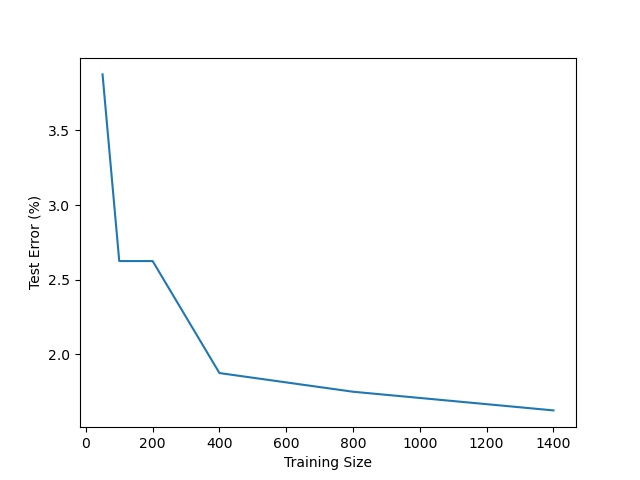
\includegraphics[width=4in,height=3.2in]{hw2_q4_c.png} 
        \caption{The test of error with respect to size of training sets} 
        \label{Fig2}
    \end{figure}
    As shown in Fig. \ref{Fig2}, we can see the the test of error with respect to size of training sets.
    It is obviously that the 1400 training set size gives us the best classification error.


\end{homeworkProblem}
\end{document}